% =====================================================================
%  ch03a.tex —— 第 3 章 Shen–Simons 微扰理论 · 章首 + §3.1
%  原书 p.101–p.110（PDF 121–130）  译者：Lead（接手）
% =====================================================================

% [原文 p.101]
\chapter{Chern--Simons 微扰理论}

本章讨论这样一类拓扑不变量：把 Chern--Simons 泛函的配分函数在其临界点（平坦联络）附近作微扰展开，由此构造出来。首先把纽结的 Vassiliev 不变量定式化，说明用迭代积分表示它的 Kontsevich 积分。其次考察 Chern--Simons 泛函在临界点附近的行为，叙述 Hessian 与 Ray--Singer 挠率的关系。由此可以窥见 Witten 不变量 $Z_k(M)$ 在 $k\to\infty$ 时渐近展开主项的形状。关于用 Feynman 图作渐近展开，先说明有限维情形的类比，再叙述由 Axelrod--Singer 构造的、基于 Chern--Simons 微扰理论的三维流形拓扑不变量。

\section{纽结的 Vassiliev 不变量与 Kontsevich 积分}

\takeaway{本节把纽结的 Vassiliev 不变量（有限阶不变量）定义为在奇异纽结上满足 $m$ 阶消失条件的不变量，并用弦图上的 4 项关系式把它的 $m$ 阶部分化为 $\Hom_{\C}(\cA_m,\C)$。Kontsevich 用 $d\log(z_i-z_j)$ 上的迭代积分给出这个空间的逆映射，从而得到不变量以迭代积分表示的通用公式。}

Vassiliev 不变量是在研究纽结全空间的 上同调 的过程中引入的。把从 $S^{1}$ 到 $S^{3}$ 的光滑映射全体的空间记作 $\cM$。设 $\Sigma$ 为 $\cM$ 中不是嵌入的映射 $f$ 全体的子集。补集 $\cM\setminus\Sigma$ 可以看作带定向的纽结全体的空间。$\cM\setminus\Sigma$ 的连通分支与纽结的类型相对应。0 次 上同调 $H^{0}(\cM\setminus\Sigma,\C)$ 可以看作取值于 $\C$ 的、带定向纽结的拓扑不变量全

% [原文 p.102]
体所成的空间。文献 [12] 中展开的 Vassiliev 的想法是：用多项式映射逼近纽结，再利用 Alexander 对偶性，把 $\cM\setminus\Sigma$ 的 上同调 的计算归结为 $\Sigma$ 的 上同调 的计算。$\Sigma$ 可以看作带奇点的纽结的集合，所以大致的想法是计算由奇点程度给出的滤过所对应的谱序列。这里没有余裕把 Vassiliev 的理论完全展开，因此只对出现在 Vassiliev 谱序列 $E_{1}$ 项中的所谓有限阶不变量作组合式的定式化。

把 $\Sigma$ 中恰有 $m$ 个横截二重点的元素 $f\colon S^{1}\to S^{3}$ 全体记作 $\cS_m$。这里横截是指：通过二重点的两条曲线的切向量线性无关。

对 $S^{3}$ 内带定向纽结的、取值于复数的拓扑不变量 $v$，如下定义「$v$ 是 $m$ 阶 Vassiliev 不变量」：考察纽结 $K$ 的投影图中 $n$ 个交叉，按 $\varepsilon_j=\pm1$（$j=1,\dots,n$）把这些交叉取为正或负所得纽结记作 $K_{\varepsilon_1\cdots\varepsilon_n}$。若 $n>m$ 时恒有
\begin{equation}
  \sum_{\varepsilon_j=\pm1,\ j=1,\dots,n}
  \varepsilon_1\cdots\varepsilon_n\, v(K_{\varepsilon_1\cdots\varepsilon_n})=0 \tag{3.1}
\end{equation}
成立，则称 $v$ 为 $m$ 阶 Vassiliev 不变量。用带二重点的纽结的语言，这个概念也可以这样表述：对 $\cS_m$ 的元素 $f$，把 $m$ 个二重点按 $\varepsilon_j=\pm 1$ 替换为正或负交叉所得纽结同样记作 $K_{\varepsilon_1\cdots\varepsilon_m}$（$\varepsilon_j=\pm1$，$j=1,\dots,m$），把 $v\colon\cM\setminus\Sigma\to\C$ 按 (3.1) 左端的值延拓到 $\bigcup_{n\ge1}\cS_n$ 上。此时，「$v$ 是 $m$ 阶 Vassiliev 不变量」等价于「$n>m$ 时 $v$ 在 $\cS_n$ 上恒为 $0$」。

把 $m$ 阶 Vassiliev 不变量全体所成的线性空间记作 $V_m$。由于 $V_m\subseteq V_{m+1}$，得到线性空间的递增列
\[
  \C=V_{0}\subseteq V_{1}\subseteq V_{2}\subseteq\cdots\subseteq V_{m}\subseteq V_{m+1}\subseteq\cdots .
\]
后面将说明，实际上 $V_{0}=V_{1}$，可见

% [原文 p.103]
1 阶 Vassiliev 不变量只有平凡者。

如图 3.1 所示，在带定向的圆周上取 $2m$ 个点、把每两个点用虚线连起来所得的图，称为\textbf{弦图}（chord diagram）。弦图按保持圆周定向的同胚相互等同。一般地，若 $v$ 是 $m$ 阶 Vassiliev 不变量，则对由 $m$ 条弦构成的弦图，如下确定一个值：如图 3.1 上方，把弦图 $\Gamma$ 中用虚线连接的两点各作等同，得到具有 $m$ 个横截二重点的 $S^{1}$ 的浸入。按上面所述，把 $v$ 延拓到带二重点的纽结上，把所得的值记作 $w(\Gamma)$。此时，对应于弦图的 $S^{1}$ 浸入并不唯一确定；但由 $v$ 是 $m$ 阶不变量这一事实要注意：$w(\Gamma)$ 不依赖于 $m$ 个二重点以外交叉的上下次序，只由弦图本身确定。把由 $m$ 条弦构成的弦图全体作为基的复向量空间记作 $\cD_m$。由上述构造得到线性映射
\[
  w\colon V_m\longrightarrow \Hom_{\C}(\cD_m,\C).
\]
为叙述这个 $w$ 所满足的关系式，先准备几个记号。如图 3.1 所示，对以圆周上用箭头标出的圆弧为端点的弦，考虑 4 种位置关系，把其余弦都一致的弦图分别记作 $S_1,S_2,S_3,S_4$。不过这里假定以带箭头的圆弧为端点的弦除此之外不存在。又如图 3.1 下方，把连结婚周上相邻两点的弦的图，称为含孤立弦的弦图。

\begin{proposition*}{3.1}
  对 $m$ 阶 Vassiliev 不变量 $v$，$w(v)$ 满足下列关系式。
  \begin{equation}
    \sum_{i=1}^{4}(-1)^{i}w(v)(S_i)=0 \tag{3.2}
  \end{equation}
  \begin{equation}
    \text{若 } S \text{ 有孤立弦，则 } w(v)(S)=0 . \tag{3.3}
  \end{equation}
\end{proposition*}

\begin{proof}
  关于关系式 (3.2)，按式 (3.1)，把 $w(v)(S_i)$ 用各自的两个二重点替换为正交叉点与负交叉点所得的 4 种图式上 $w(v)$ 的值的交代和表示，即可立刻得到。关系式 (3.3) 由不变量 $v$ 是纽结的不变量、不依赖于 framing 这一事实得到。
\end{proof}

% [原文 p.104]
\begin{figure}[htbp]
  \centering
  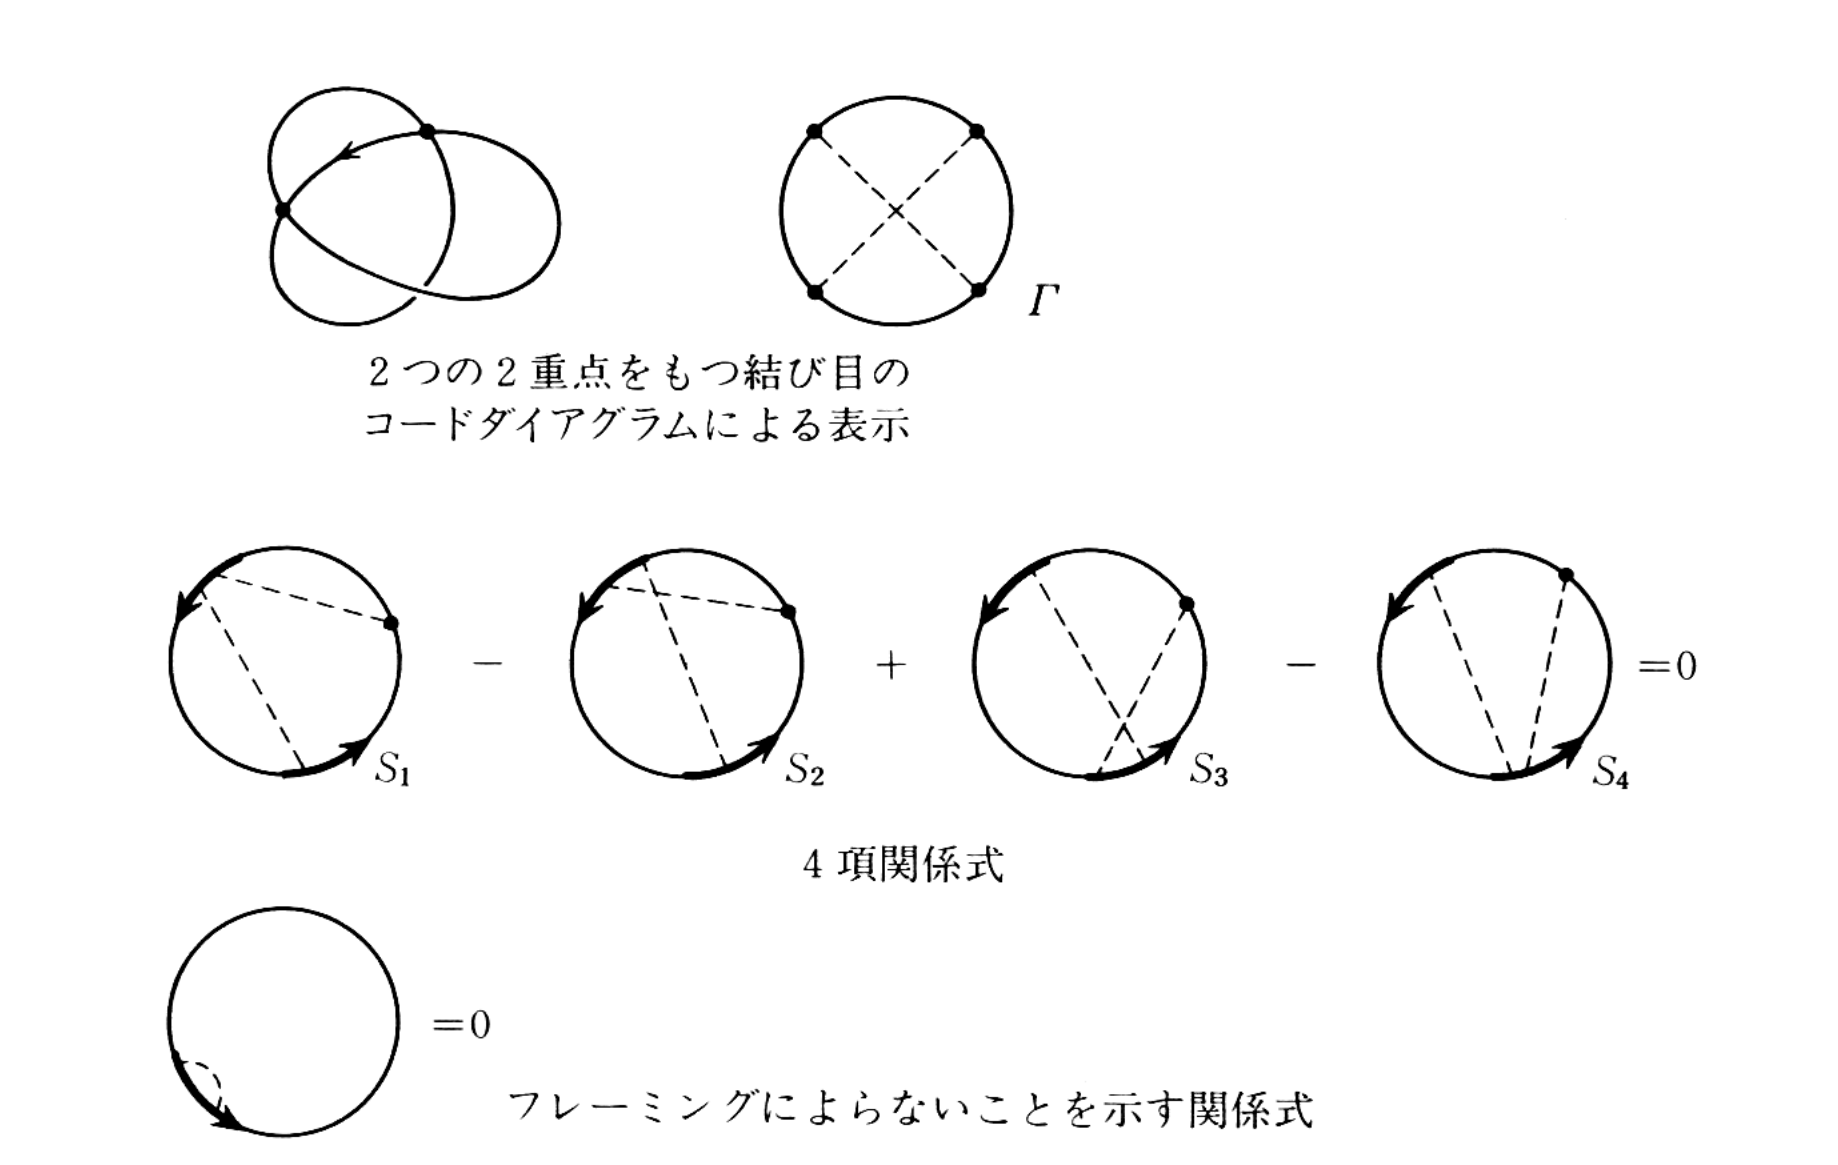
\includegraphics[width=0.82\textwidth]{figures/fig3.1.png}
  \figtitle{3.1}{上：带两个二重点的纽结及其弦图表示（$\Gamma$）；中：4 项关系式（$S_1-S_2+S_3-S_4=0$）；下：表示不依赖 framing 的关系式。（原书 p.104）}
\end{figure}

关系式 (3.2) 称为 \textbf{4 项关系式}（4 term relation）。把线性空间 $\cD_m$ 用命题 3.1 中出现的两种关系式左端所生成的部分空间作商所得的空间记作 $\cA_m$。由命题 3.1，从上述构造得到单射
\begin{equation}
  V_m/V_{m-1}\longrightarrow \Hom_{\C}(\cA_m,\C). \tag{3.4}
\end{equation}
由此，特别可知 $V_m/V_{m-1}$ 是有限维复线性空间。又，只有 1 条弦的弦图含孤立弦，故 $\cA_1=0$，从而也能确认 $V_0=V_1$。

Kontsevich 用迭代积分构造了这个逆映射，并证明了 (3.4) 是同构。下面叙述 Kontsevich 的迭代积分。这里从「Kontsevich 的迭代积分是辫子的 Chen 迭代积分的自然推广」这一观点来说明。与 2.1 节同样，把复平面 $\C$ 的相异

% [原文 p.105]
$n$ 个点的构形空间记作 $\Conf_n(\C)$。$\Conf_n(\C)$ 上的微分形式 $\omega_{ij}$ 定义为
\[
  \omega_{ij}=d\log(z_i-z_j)=\frac{dz_i-dz_j}{z_i-z_j},\qquad i\ne j .
\]
进而，在与 2.1 节相同的状况下，对复参数 $\kappa$ 令
\[
  \omega=\frac{1}{\kappa}\sum_{1\le i<j\le n}\Omega_{ij}\,\omega_{ij},
\]
考虑全微分方程
\begin{equation}
  d\Phi=\omega\Phi . \tag{3.5}
\end{equation}
KZ 方程的单值表示，作为 $\omega$ 所定联络的和乐得到；它的一个表示由 Chen 迭代积分之和给出。也就是说，把全微分方程 (3.5) 沿道路 $\gamma(t)$（$0\le t\le 1$）化为积分方程、再用逐次迭代法求解，则满足 $\Phi(\gamma(0))=I$ 的全微分方程 (3.5) 的解可用
\begin{equation}
  J_m(\gamma)=\int_{\gamma}\underbrace{\omega\cdots\omega}_{m} \tag{3.6}
\end{equation}
表示为
\begin{equation}
  \Phi(\gamma(1))=I+\sum_{m=1}^{\infty}J_m(\gamma). \tag{3.7}
\end{equation}
这里 $J_m(\gamma)$ 是 $m$ 阶的\textbf{迭代积分}（iterated integral），定义如下。一般地，取 $\omega_1,\dots,\omega_m$ 为一次微分形式，把它们沿道路 $\gamma$ 的拉回写成 $\alpha_1(t)\,dt,\dots,\alpha_m(t)\,dt$（$0\le t\le1$），则迭代积分定义为
\begin{equation}
  \int_{\gamma}\omega_1\cdots\omega_m
  =\int_{0\le t_1\le\cdots\le t_m\le 1}
  \alpha_1(t_1)\cdots\alpha_m(t_m)\,dt_1\cdots dt_m . \tag{3.8}
\end{equation}
KZ 联络的曲率为 $0$ 这件事，由 $\Omega_{ij}$ 之间的下列关系式
\begin{equation}
  [\Omega_{ij}+\Omega_{jk},\,\Omega_{ik}]=0
  \qquad (i,j,k\ \text{互不相同}) \tag{3.9}
\end{equation}

% [原文 p.106]
\begin{equation}
  [\Omega_{ij},\,\Omega_{kl}]=0
  \qquad (i,j,k,l\ \text{互不相同}) \tag{3.10}
\end{equation}
来保证。注意到这一点，引入非交换的形式变量 $X_{ij}$（$1\le i\ne j\le n$），用迭代积分把 KZ 方程单值表示的通用形式表示为幂级数。首先，把变量 $X_{ij}$（$1\le i\ne j\le n$）在 $\C$ 上的非交换形式幂级数环，用 $X_{ij}-X_{ji}$ 及
\begin{equation}
  [X_{ij}+X_{jk},\,X_{ik}] \qquad (i,j,k\ \text{互不相同}) \tag{3.11}
\end{equation}
\begin{equation}
  [X_{ij},\,X_{kl}] \qquad (i,j,k,l\ \text{互不相同}) \tag{3.12}
\end{equation}
所生成的双边理想作商所得的 $\C$ 代数记作 $A_n$。以 $\kappa$ 为参数，考虑取值于 $A_n$ 的一次微分形式
\[
  \tilde\omega=\frac{1}{\kappa}\sum_{1\le i<j\le n}X_{ij}\,\omega_{ij}.
\]
与式 (3.7) 同样，令
\[
  \tilde\theta(\gamma)=1+\sum_{m=1}^{\infty}\int_{\gamma}\underbrace{\tilde\omega\cdots\tilde\omega}_{m},
\]
则由 (3.11)、(3.12)，$\tilde\omega$ 确定平坦联络，故 $\tilde\theta(\gamma)$ 只依赖于 $\gamma$ 的同伦类，得到从纯辫群 $P_n$ 出发的同态
\[
  \tilde\theta\colon P_n\longrightarrow A_n .
\]
这里，对 $\gamma\in P_n$，$\tilde\theta(\gamma)$ 是关于变量 $X_{ij}$ 的幂级数，其系数由对数微分形式 $\omega_{ij}$ 的迭代积分给出。又，KZ 方程的单值表示，可以通过把矩阵 $\Omega_{ij}$ 代入变量 $X_{ij}$ 得到。在这个意义上，$\tilde\theta$ 也可以理解为 KZ 方程单值表示的通用表示。此外还可知道：联络曲率为 $0$ 所必需的关系式 (3.9)，与 Vassiliev 不变量的讨论中出现的 4 项关系式本质上是同一个东西。

把微分形式 $\omega_{ij}$ 沿 $\Conf_n(\C)$ 的道路 $\gamma(t)=(z_1(t),\dots,z_n(t))$ 的拉回表示为
\begin{equation}
  \omega_{ij}(t)=\frac{dz_i(t)-dz_j(t)}{z_i(t)-z_j(t)} . \tag{3.13}
\end{equation}
把上面 $\tilde\theta(\gamma)$ 的迭代积分表示具体写出，则

% [原文 p.107]
\begin{equation}
  \sum_{m=0}^{\infty}\int_{0\le t_1\le t_2\le\cdots\le t_m\le 1}
  \frac{1}{\kappa^{m}}\sum_{P}X_{i_1j_1}\cdots X_{i_mj_m}
  \bigwedge_{k=1}^{m}\omega_{i_kj_k}(t_k) \tag{3.14}
\end{equation}
其中 $P=(i_1j_1,\dots,i_mj_m)$ 遍历满足 $1\le i_1<j_1\le n$、$\dots$、$1\le i_m<j_m\le n$ 的所有组 $(i_1,j_1),\dots,(i_m,j_m)$。

Kontsevich 把这一表示推广到纽结的情形，得到了纽结的 Vassiliev 不变量的通用积分表示。如图 3.2，考虑 $\C\times\R$ 内带定向的纽结 $K$。以 $\R$ 方向的坐标函数为 $t$，假定 $K$ 上函数 $t$ 的临界点全都非退化，即高度函数是纽结 $K$ 上的 Morse 函数。把连结高度函数 $t$ 的极大点与极小点的曲线记作 $z_i(t)$。图 3.2 中 $i=1,\dots,4$。考虑迭代积分
\begin{equation}
\begin{aligned}
  Z_m(K)=\frac{1}{(2\pi\sqrt{-1})^{m}}
  \int_{t_1<t_2<\cdots<t_m}\sum_{P}(-1)^{\varepsilon(P)}D_{P}
  \bigwedge_{k=1}^{m}\omega_{i_kj_k}(t_k)
\end{aligned}
\tag{3.15}
\end{equation}
这里 $P=(i_1j_1,\dots,i_mj_m)$ 表示在 $t_1<\cdots<t_m$ 各层上各选两条曲线 $z_i(t)$ 的方法，和取遍所有这样的选法。每个 $P$ 如图 3.2 对应由 $m$ 条弦构成的图 $D_P$，把它按关系式 (3.2)、(3.3) 视为 $\cA_m$ 的元素。又 $\varepsilon(P)$ 表示 $P$ 中出现的虚线的端点处 $K$ 的定向朝下的个数。积分 (3.15) 被视为 $\cA_m$ 的元素，称为 \textbf{Kontsevich 积分}。

\begin{lemma}{3.2}
  积分 (3.15) 作为 $\cA_m$ 的元素收敛，并且在纽结沿水平方向的同痕移动下不变。
\end{lemma}

由关系式 (3.3)，这个积分在极大点、极小点处不发散，恒取有限值。又，4 项关系式 (3.2) 对应 KZ 方程的可积条件 (3.9)，故把纽结沿水平方向移动时值不变。令

% [原文 p.108]
\begin{equation}
  Z(K)=\sum_{m=0}^{\infty}Z_m(K)\in\prod_{m=0}^{\infty}\cA_m . \tag{3.16}
\end{equation}
这里 $\prod_{m=0}^{\infty}\cA_m$ 表示无限直积。这样还不能对图 2.11 的两个临界点的对消操作保持不变，故与 2.2 节的讨论同样，作如下修正。取 $K_0$ 为图 2.11 右侧那样的、有 4 个临界点的平凡纽结，用 $Z(K_0)$ 令
\begin{equation}
  \tilde Z(K)=Z(K)\cdot Z(K_0)^{-\mu(K)+1} \tag{3.17}
\end{equation}
其中 $\mu(K)$ 表示 $K$ 的极大点个数。在无限直积 $\prod_{m=0}^{\infty}\cA_m$ 中表为
\[
  \tilde Z(K)=\sum_{m=0}^{\infty}\tilde Z_m(K),\qquad \tilde Z_m(K)\in\cA_m .
\]
如此便得到 Kontsevich 的下列定理。

\begin{theorem}{3.3}
  （Kontsevich）$\tilde Z(K)$ 是取值于 $\prod_{m=0}^{\infty}\cA_m$ 的纽结拓扑不变量。又，$\tilde Z_m(K)$ 是取值于 $\cA_m$ 的 $m$ 阶拓扑不变量。
\end{theorem}

\begin{figure}[htbp]
  \centering
  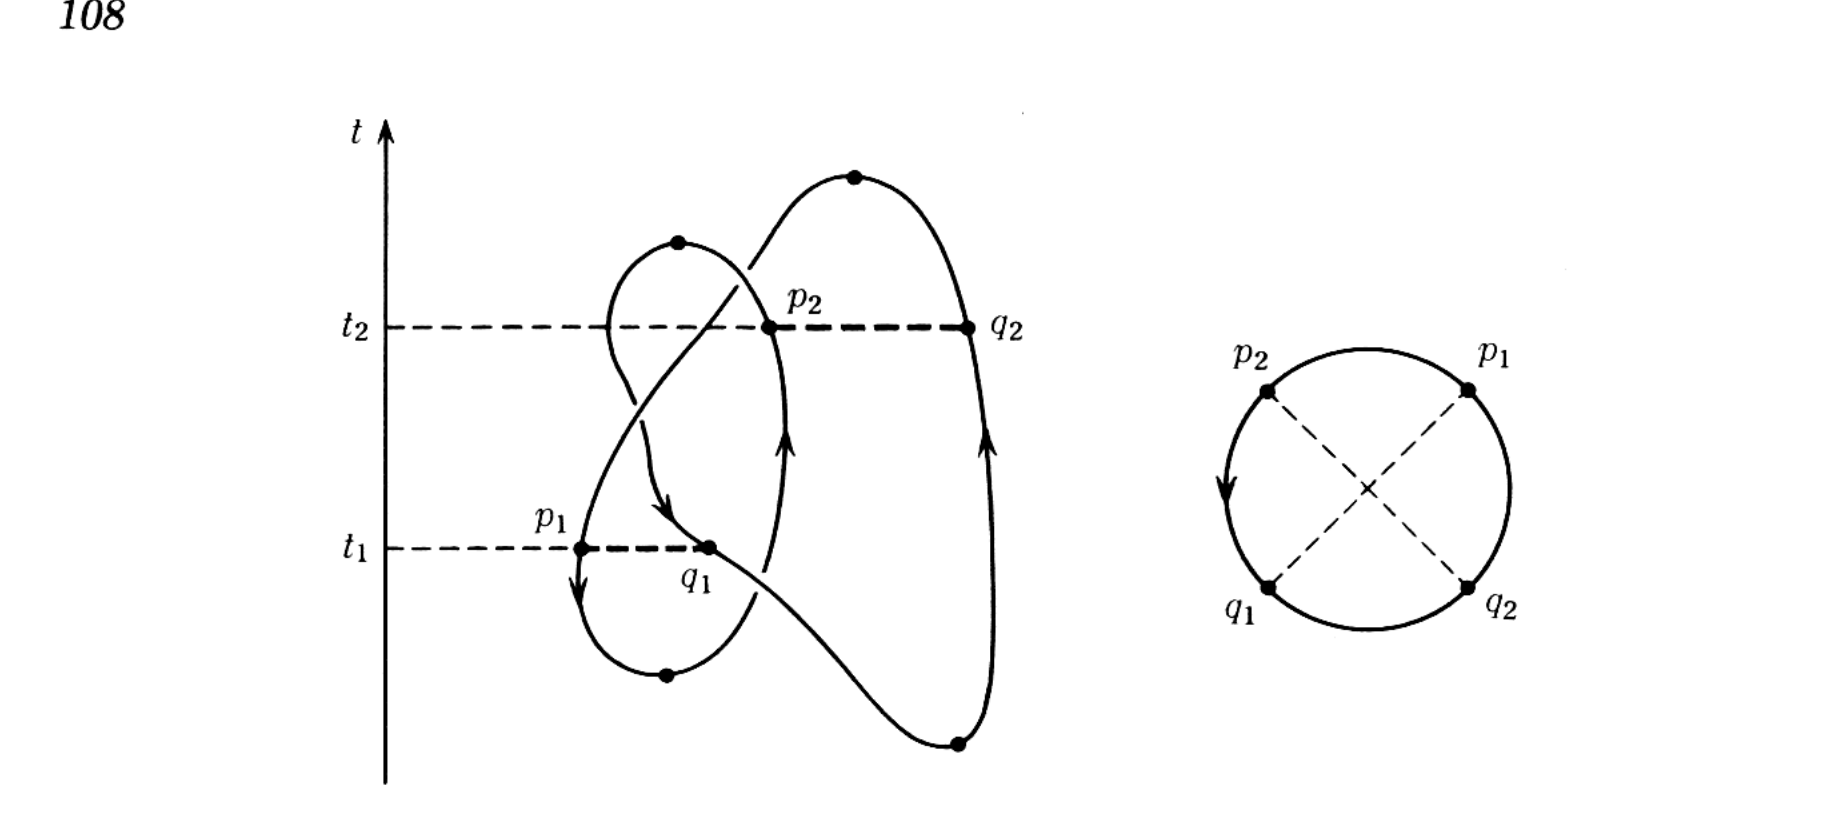
\includegraphics[width=0.78\textwidth]{figures/fig3.2.png}
  \figtitle{3.2}{$\C\times\R$ 内的纽结 $K$，以及由层 $t_1,t_2$ 上的选法所得的弦图 $D_P$。（原书 p.108）}
\end{figure}

链环的 \textbf{Conway 多项式}是带定向链环的不变量，由拆接关系式
\[
  \nabla_{L_+}-\nabla_{L_-}=z\nabla_{L_0},\qquad \nabla_{\bigcirc}=1
\]
刻画。$\nabla_L$ 是以为 $z$ 变量的多项式。Vassiliev 不变量的

% [原文 p.109]
定义对带定向链环也容易推广；把 $\nabla_L$ 中 $z^{k}$ 的系数记作 $a_k(L)$，则可立刻确认 $a_k$ 是 $k$ 阶不变量。特别地，注意纽结 $K$ 的 2 阶不变量，由式 (3.17) 的 2 次项得到
\begin{equation}
\begin{aligned}
  \frac{1}{4\pi^{2}}\int_{t_1<t_2}
  \sum_{P}(-1)^{\varepsilon(P)}D_{P}\,\omega_{i_1j_1}(t_1)\wedge\omega_{i_2j_2}(t_2)
  +\frac{1}{24}\mu(K)-\frac{1}{24}
\end{aligned}
\tag{3.18}
\end{equation}
当 $D_P$ 为图 3.2 右侧的图时取 $D_P=1$，否则取 $0$；此时可以证明积分 (3.18) 是取整数值的纽结拓扑不变量，与 Conway 多项式的 2 次系数一致。

上述 Conway 多项式 2 次系数的积分表示，用到了 $Z(K_0)$ 的 2 次项的计算。这个计算中出现了图 3.3 右侧所示的 $d\log t$ 与 $d\log(1-t)$ 的迭代积分。它可用 \textbf{二重对数函数}（dilogarithm）表为
\[
  \int_{0}^{1}\frac{\log(1-t)}{t}\,dt=-\frac{\pi^{2}}{6}.
\]
$Z(K_0)$ 的高次项中出现 $d\log t$ 与 $d\log(1-t)$ 的高次迭代积分，它可用\textbf{多重 zeta 函数}（multiple zeta function）
\[
  \zeta(s_1,s_2,\dots,s_k)=\sum_{0<m_1<m_2<\cdots<m_k}\frac{1}{m_1^{s_1}\cdots m_k^{s_k}}
\]
的特殊值表示。这里 $m_1,\dots,m_k$ 是正整数。

$\cA_m$ 的对偶空间的元素称为\textbf{权系统}（weight system）。由定理 3.3，给定权系统，就能构造纽结的拓扑不变量。构造权系统的一种方法，是用半单 Lie 代数 $\fg$ 及其表示 $r\colon\fg\to\End(V)$。具体地说，如图 3.3 左侧所示，把弦图分解为两种基本构成要素，对它们分别对应
\[
  \frac{1}{\kappa}\Omega=\frac{1}{\kappa}\sum_{\mu}I_{\mu}\otimes I_{\mu}\in\fg\otimes\fg
\]
以及对应于表示 $r$ 的 $\fg^{*}\otimes V^{*}\otimes V$ 的元素。这里 $\{I_\mu\}$ 是关于 $\fg$ 的 Cartan--Killing 型的正规正交基。可以确认：按弦图缩并这些张量所得的标量满足 4 项关系式。对这个标量

% [原文 p.110]
\begin{figure}[htbp]
  \centering
  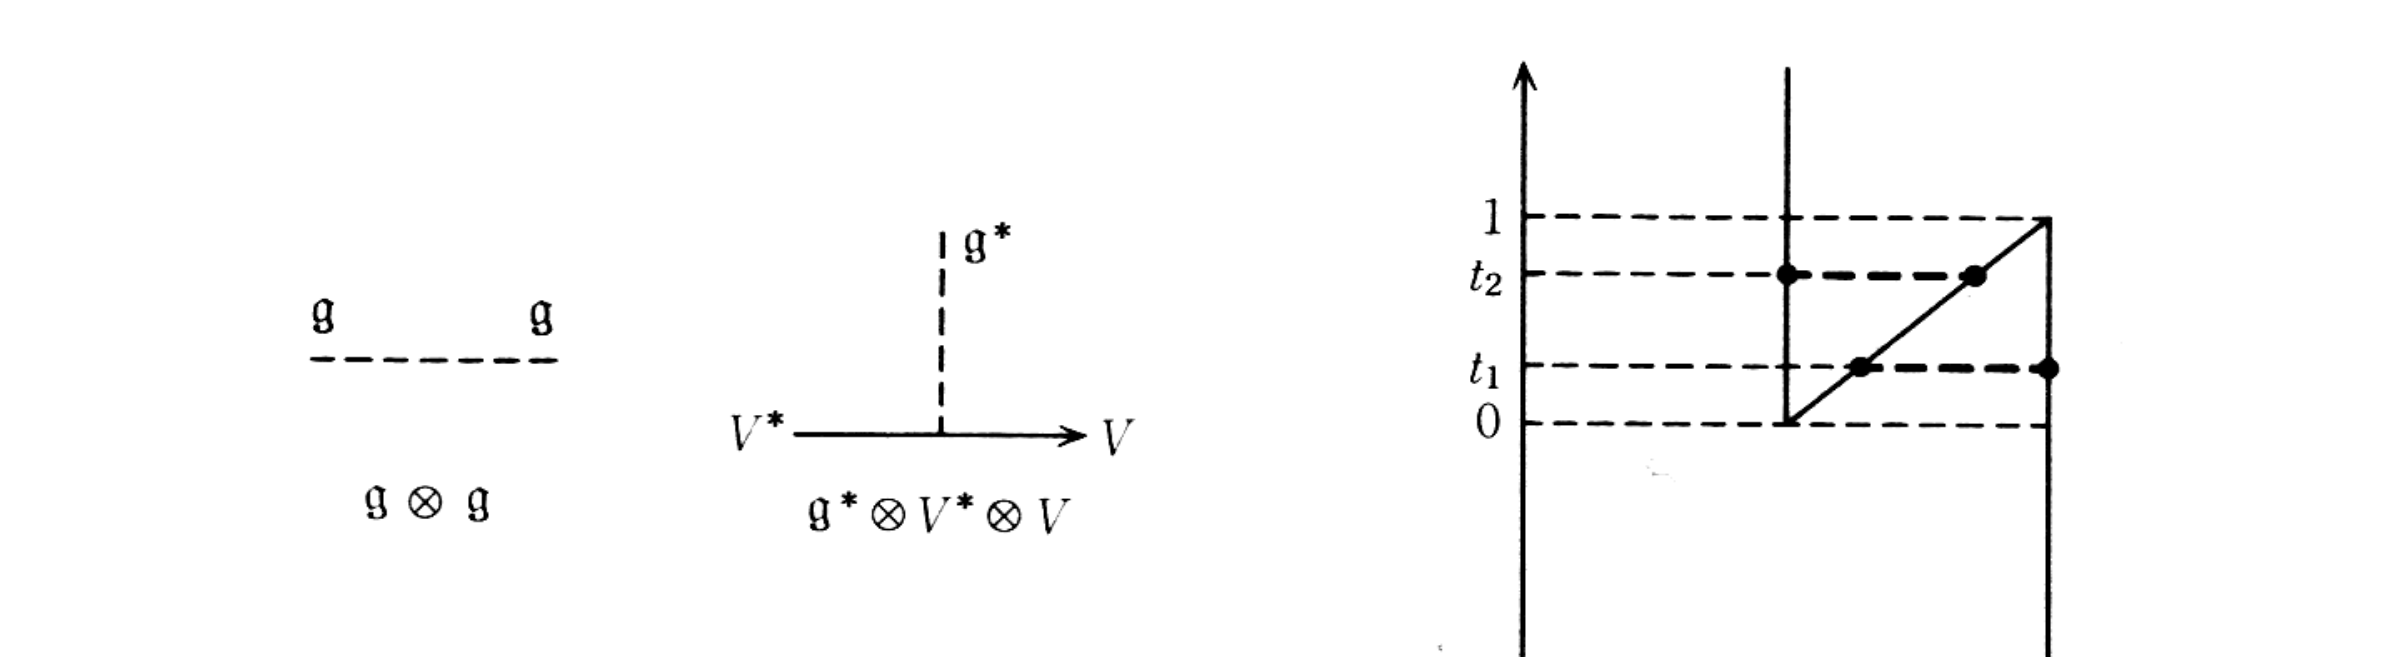
\includegraphics[width=0.92\textwidth]{figures/fig3.3.png}
  \figtitle{3.3}{左：由 Lie 代数 $\fg$ 及其表示 $V$ 构造权系统；右：$Z(K_0)$ 的 2 次项的计算。（原书 p.110）}
\end{figure}

再按关系式 (3.3) 作归一化，所得的就是所求的权系统。

如定理 2.3 之后所述，在 $\fg=\mathfrak{sl}_m(\C)$ 及其 $m$ 维表示的情形，辫群的单值表示成为 Iwahori--Hecke 代数的表示。在这种状况下构造上述权系统，对所得不变量计算拆接关系式，可知不变量是 2 变量 Jones 多项式 $P(x,y)$ 在
\[
  x=q^{\frac{m}{2}},\qquad y=q^{-\frac{1}{2}}-q^{\frac{1}{2}}
\]
处取值所得者。这里 $q=\exp(2\pi\sqrt{-1}/\kappa)$；2 变量 Jones 多项式由拆接关系式
\[
  x^{-1}P_{L_+}-xP_{L_-}=yP_{L_0},\qquad P_{\bigcirc}=1
\]
刻画。由此，归一化项 $Z(K_0)$ 为
\[
  Z(K_0)=\frac{m\,(q^{1/2}-q^{-1/2})}{q^{m/2}-q^{-m/2}} .
\]
文献 [38] 中，用这样的考察把上述 $Z(K_0)$ 与 $d\log t$、$d\log(1-t)$ 的迭代积分表示相比较，求出了多重 zeta 函数特殊值之间的关系式。例如可证明
\[
  \Bigl(\frac{1}{2^{2n-2}}-1\Bigr)\zeta(2n)-\zeta(1,2n-1)+\cdots
  +\zeta(\underbrace{1,\dots,1}_{2n-2},2)=0 .
\]

% [Tutor Note: 本节把三个层次分得很清楚：$V_m$（纽结不变量）$\to$ $\cA_m$（弦图模 4 项关系与孤立弦关系）$\to$ 权系统（$\cA_m^{*}$ 的元素）。定理 3.3 说 Kontsevich 积分给出 $V_m \to \cA_m^{*}$ 的逆映射，所以「所有 Vassiliev 不变量」与「所有权系统」一一对应，这是 §3.2 构造 $Z_k(M)$ 渐近展开的出发点。]

% [Tutor Note: (3.1) 的求和约定容易读错：$\varepsilon_j$ 取 $\pm1$ 共有 $2^{n}$ 项，$\varepsilon_1\cdots\varepsilon_n$ 是符号因子；$n>m$ 时恒为零正是「$m$ 阶不变量对 $m+1$ 个二重点的符号和为零」，与 (3.2) 的 4 项关系式是同一件事的两种写法。]

% [Tutor Note: (3.17) 的指数是 $-\mu(K)+1$（$\mu(K)$ 为极大点个数），不是 $-\mu(K)-1$。这是因为 $(2\pi\sqrt{-1})^{-m}$ 的归一化与 $K_0$ 的极大点计数一起吸收掉了 framing 与临界点对消的差异；页图 p.108 已逐字复核。]

% [Tutor Note: (3.15) 的 $D_P$ 只在「$D_P$ 等于图 3.2 右侧的图」时取 1，它是把弦图映为 $\cA_m$ 中元素后的系数；$\varepsilon(P)$ 数的是虚线的端点中「$K$ 的定向朝下」的个数，方向颠倒会整体变号，核对时以页图 p.107 的图为准。]

% [Tutor Note: $Z(K_0)$ 的公式里 $m$ 同时出现在分子（$m(q^{1/2}-q^{-1/2})$）与分母的指数（$q^{m/2}-q^{-m/2}$），其中分子的 $m$ 来自 $m$ 维表示 $\mathfrak{sl}_m$ 的维数，不要与弦的条数 $m$ 混淆（本例中两者恰好同号）。]

% CHUNK ch03a DONE
